\documentclass[twoside]{book}

% Packages required by doxygen
\usepackage{fixltx2e}
\usepackage{calc}
\usepackage{doxygen}
\usepackage[export]{adjustbox} % also loads graphicx
\usepackage{graphicx}
\usepackage[utf8]{inputenc}
\usepackage{makeidx}
\usepackage{multicol}
\usepackage{multirow}
\PassOptionsToPackage{warn}{textcomp}
\usepackage{textcomp}
\usepackage[nointegrals]{wasysym}
\usepackage[table]{xcolor}

% Font selection
\usepackage[T1]{fontenc}
\usepackage[scaled=.90]{helvet}
\usepackage{courier}
\usepackage{amssymb}
\usepackage{sectsty}
\renewcommand{\familydefault}{\sfdefault}
\allsectionsfont{%
  \fontseries{bc}\selectfont%
  \color{darkgray}%
}
\renewcommand{\DoxyLabelFont}{%
  \fontseries{bc}\selectfont%
  \color{darkgray}%
}
\newcommand{\+}{\discretionary{\mbox{\scriptsize$\hookleftarrow$}}{}{}}

% Page & text layout
\usepackage{geometry}
\geometry{%
  a4paper,%
  top=2.5cm,%
  bottom=2.5cm,%
  left=2.5cm,%
  right=2.5cm%
}
\tolerance=750
\hfuzz=15pt
\hbadness=750
\setlength{\emergencystretch}{15pt}
\setlength{\parindent}{0cm}
\setlength{\parskip}{3ex plus 2ex minus 2ex}
\makeatletter
\renewcommand{\paragraph}{%
  \@startsection{paragraph}{4}{0ex}{-1.0ex}{1.0ex}{%
    \normalfont\normalsize\bfseries\SS@parafont%
  }%
}
\renewcommand{\subparagraph}{%
  \@startsection{subparagraph}{5}{0ex}{-1.0ex}{1.0ex}{%
    \normalfont\normalsize\bfseries\SS@subparafont%
  }%
}
\makeatother

% Headers & footers
\usepackage{fancyhdr}
\pagestyle{fancyplain}
\fancyhead[LE]{\fancyplain{}{\bfseries\thepage}}
\fancyhead[CE]{\fancyplain{}{}}
\fancyhead[RE]{\fancyplain{}{\bfseries\leftmark}}
\fancyhead[LO]{\fancyplain{}{\bfseries\rightmark}}
\fancyhead[CO]{\fancyplain{}{}}
\fancyhead[RO]{\fancyplain{}{\bfseries\thepage}}
\fancyfoot[LE]{\fancyplain{}{}}
\fancyfoot[CE]{\fancyplain{}{}}
\fancyfoot[RE]{\fancyplain{}{\bfseries\scriptsize Generated by Doxygen }}
\fancyfoot[LO]{\fancyplain{}{\bfseries\scriptsize Generated by Doxygen }}
\fancyfoot[CO]{\fancyplain{}{}}
\fancyfoot[RO]{\fancyplain{}{}}
\renewcommand{\footrulewidth}{0.4pt}
\renewcommand{\chaptermark}[1]{%
  \markboth{#1}{}%
}
\renewcommand{\sectionmark}[1]{%
  \markright{\thesection\ #1}%
}

% Indices & bibliography
\usepackage{natbib}
\usepackage[titles]{tocloft}
\setcounter{tocdepth}{3}
\setcounter{secnumdepth}{5}
\makeindex

% Hyperlinks (required, but should be loaded last)
\usepackage{ifpdf}
\ifpdf
  \usepackage[pdftex,pagebackref=true]{hyperref}
\else
  \usepackage[ps2pdf,pagebackref=true]{hyperref}
\fi
\hypersetup{%
  colorlinks=true,%
  linkcolor=blue,%
  citecolor=blue,%
  unicode%
}

% Custom commands
\newcommand{\clearemptydoublepage}{%
  \newpage{\pagestyle{empty}\cleardoublepage}%
}

\usepackage{caption}
\captionsetup{labelsep=space,justification=centering,font={bf},singlelinecheck=off,skip=4pt,position=top}

%===== C O N T E N T S =====

\begin{document}

% Titlepage & ToC
\hypersetup{pageanchor=false,
             bookmarksnumbered=true,
             pdfencoding=unicode
            }
\pagenumbering{alph}
\begin{titlepage}
\vspace*{7cm}
\begin{center}%
{\Large Send\+Help Snake 2.0 }\\
\vspace*{1cm}
{\large Generated by Doxygen 1.8.13}\\
\end{center}
\end{titlepage}
\clearemptydoublepage
\pagenumbering{roman}
\tableofcontents
\clearemptydoublepage
\pagenumbering{arabic}
\hypersetup{pageanchor=true}

%--- Begin generated contents ---
\chapter{Hierarchical Index}
\section{Class Hierarchy}
This inheritance list is sorted roughly, but not completely, alphabetically\+:\begin{DoxyCompactList}
\item Action\+Listener\begin{DoxyCompactList}
\item \contentsline{section}{Board}{\pageref{class_board}}{}
\end{DoxyCompactList}
\item J\+Frame\begin{DoxyCompactList}
\item \contentsline{section}{Snake}{\pageref{class_snake}}{}
\end{DoxyCompactList}
\item J\+Panel\begin{DoxyCompactList}
\item \contentsline{section}{Board}{\pageref{class_board}}{}
\end{DoxyCompactList}
\end{DoxyCompactList}

\chapter{Class Index}
\section{Class List}
Here are the classes, structs, unions and interfaces with brief descriptions\+:\begin{DoxyCompactList}
\item\contentsline{section}{\hyperlink{class_board}{Board} }{\pageref{class_board}}{}
\item\contentsline{section}{\hyperlink{class_snake}{Snake} }{\pageref{class_snake}}{}
\end{DoxyCompactList}

\chapter{Class Documentation}
\hypertarget{class_board}{}\section{Board Class Reference}
\label{class_board}\index{Board@{Board}}
Inheritance diagram for Board\+:\begin{figure}[H]
\begin{center}
\leavevmode
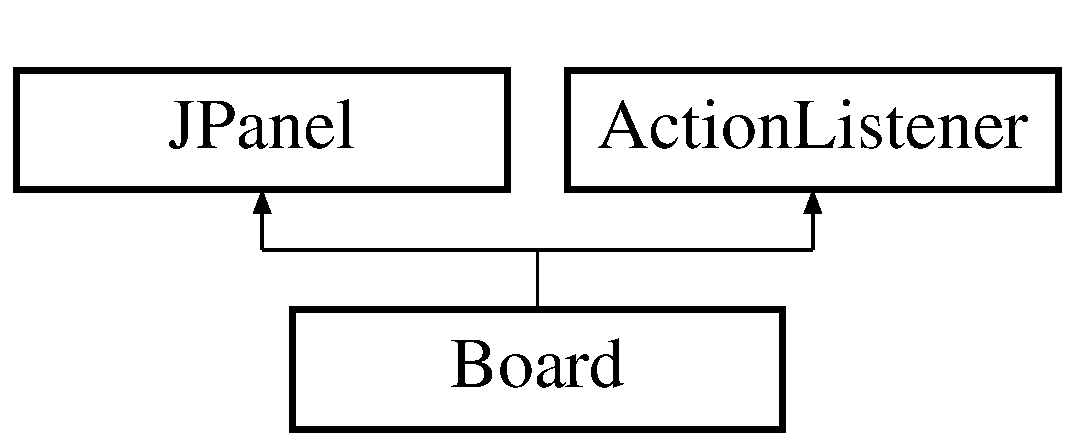
\includegraphics[height=2.000000cm]{class_board}
\end{center}
\end{figure}
\subsection*{Public Member Functions}
\begin{DoxyCompactItemize}
\item 
\hyperlink{class_board_ab5e792f71e2fbff747bf7b52859f2a98}{Board} ()
\item 
void \hyperlink{class_board_aa3a8c18495cd2acb36b6227a008861a0}{set\+Delay} (int delay)
\item 
void \hyperlink{class_board_a2a8e54034cf6e22a174e668b54d57368}{load\+Images} ()
\item 
void \hyperlink{class_board_a510b3c25a75fbfdc3a2d4bd0660cf958}{reset} ()
\item 
void \hyperlink{class_board_a05f7155d1fb7219fa0081ddbe68bdcad}{paint\+Component} (Graphics g)
\item 
void \hyperlink{class_board_a1bd348eafebfa5845ff0d8ed9c11f341}{check\+Pellet} ()
\item 
void \hyperlink{class_board_a916df1693e14ee32843e7d2a6ed1b1b6}{move} ()
\item 
void \hyperlink{class_board_a8eef2b7fbeb8fb80037c793ca2d04e8f}{check\+Collision} ()  throws Interrupted\+Exception 
\item 
void \hyperlink{class_board_a93eeb133b26a224fe23447478700d8c7}{locate\+Pellet} ()
\item 
void \hyperlink{class_board_ae4495c39178937ad35a9838e816e8953}{action\+Performed} (Action\+Event e)
\end{DoxyCompactItemize}
\subsection*{Public Attributes}
\begin{DoxyCompactItemize}
\item 
final int \hyperlink{class_board_a26390bed1bf2786b56e6ce5c8bdfe384}{B\+O\+A\+R\+D\+\_\+\+W\+I\+D\+TH} = 300
\item 
final int \hyperlink{class_board_a17a48c777b0c08986dd2db8837b1199d}{B\+O\+A\+R\+D\+\_\+\+H\+E\+I\+G\+HT} = 300
\item 
final int \hyperlink{class_board_a142327cbac30c9c8831b197cdd2e9a36}{D\+O\+T\+\_\+\+S\+I\+ZE} = 10
\item 
final int \hyperlink{class_board_afc3dba6349ee431f748fdcaee99b78b7}{A\+L\+L\+\_\+\+D\+O\+TS} = 900
\item 
final int \hyperlink{class_board_a7e683d47d45e3734833860cda1993366}{R\+A\+N\+D\+\_\+\+P\+OS} = 29
\item 
final int \hyperlink{class_board_a05fa7c307d2fc9f2813a728a85d1dad4}{D\+E\+L\+AY} = 140
\item 
final int \hyperlink{class_board_a1644d1bf67cadaa59812ec1b5d9d5a19}{x} \mbox{[}$\,$\mbox{]} = new int\mbox{[}\hyperlink{class_board_afc3dba6349ee431f748fdcaee99b78b7}{A\+L\+L\+\_\+\+D\+O\+TS}\mbox{]}
\item 
final int \hyperlink{class_board_a8bcec6f1642775fa45aa60e0710732a4}{y} \mbox{[}$\,$\mbox{]} = new int\mbox{[}\hyperlink{class_board_afc3dba6349ee431f748fdcaee99b78b7}{A\+L\+L\+\_\+\+D\+O\+TS}\mbox{]}
\item 
int \hyperlink{class_board_ac2d4eeff3a96ccb227e8cc38ff803d50}{dots}
\item 
int \hyperlink{class_board_ad10f2e196700bf4db295150b320b1f07}{pellet\+\_\+x}
\item 
int \hyperlink{class_board_a9ef3d56a9df039b5b1c6a7172e77d233}{pellet\+\_\+y}
\item 
Random \hyperlink{class_board_a437c36e144698e50f2a842d4b60979e3}{rand} = new Random()
\item 
boolean \hyperlink{class_board_a57b230f404f9f86d8ed741d25e8dcfc3}{speedup\+Pellet} = false
\item 
boolean \hyperlink{class_board_a79cef3a39a5160aa365ab9e37a768850}{slowdown\+Pellet} = false
\item 
boolean \hyperlink{class_board_add2714db81c1d069077b60f04efecf58}{collision\+Pellet} = false
\item 
boolean \hyperlink{class_board_ae1480c275ddcb277be70a914e5f90da6}{collision\+Active} = false
\item 
long \hyperlink{class_board_a91e4464171d80a72609d5d2f25954d7b}{step\+Count} = 0
\item 
long \hyperlink{class_board_a74f7919c59b8bd512e8ff8a922583822}{immunity\+Count} = 0
\item 
boolean \hyperlink{class_board_a07aa50c4b704777f8693a35b319ada03}{left\+Direction} = false
\item 
boolean \hyperlink{class_board_a07dcadb0e102900ec4110e679e6e10f1}{right\+Direction} = true
\item 
boolean \hyperlink{class_board_a91c8cf23e650424074cb0cd1638541f8}{up\+Direction} = false
\item 
boolean \hyperlink{class_board_a2c4b39d098ee72bb293cbc75ba7c3ace}{down\+Direction} = false
\item 
boolean \hyperlink{class_board_ab0bb999b1b53db2a2d157003dece54ab}{in\+Game} = true
\item 
Timer \hyperlink{class_board_adeea39bf09dfd689ac9396d7c6d95995}{timer}
\item 
Image \hyperlink{class_board_a3d149787c3692d5d5ff0e14f31c4cf9a}{ball}
\item 
Image \hyperlink{class_board_a9fd625fd3b6a4cd34d32e9ecc9c7163f}{pellet}
\item 
Image \hyperlink{class_board_aa1544ac7c813a0a8ba3aec1e46c60971}{head}
\item 
Image \hyperlink{class_board_a0c27edfc2944b6ebbc34e7f041ab3bec}{speedup}
\item 
Image \hyperlink{class_board_ac831f1556734f69a7d70fe4e8725079c}{slowdown}
\item 
Image \hyperlink{class_board_a81bb96225cd77943f0fa0c3792f52422}{collision}
\end{DoxyCompactItemize}


\subsection{Constructor \& Destructor Documentation}
\mbox{\Hypertarget{class_board_ab5e792f71e2fbff747bf7b52859f2a98}\label{class_board_ab5e792f71e2fbff747bf7b52859f2a98}} 
\index{Board@{Board}!Board@{Board}}
\index{Board@{Board}!Board@{Board}}
\subsubsection{\texorpdfstring{Board()}{Board()}}
{\footnotesize\ttfamily Board.\+Board (\begin{DoxyParamCaption}{ }\end{DoxyParamCaption})}

Constructor for \hyperlink{class_board}{Board}.

out \+:= self 

\subsection{Member Function Documentation}
\mbox{\Hypertarget{class_board_ae4495c39178937ad35a9838e816e8953}\label{class_board_ae4495c39178937ad35a9838e816e8953}} 
\index{Board@{Board}!action\+Performed@{action\+Performed}}
\index{action\+Performed@{action\+Performed}!Board@{Board}}
\subsubsection{\texorpdfstring{action\+Performed()}{actionPerformed()}}
{\footnotesize\ttfamily void Board.\+action\+Performed (\begin{DoxyParamCaption}\item[{Action\+Event}]{e }\end{DoxyParamCaption})}

Called whenever an action occurs. If the game is currently running, checks if pellet was consumed by the snake, checks if collision has occured and finally moves the snake. Repaints the scene afterwards.


\begin{DoxyParams}{Parameters}
{\em e} & Action\+Event object \\
\hline
\end{DoxyParams}
\mbox{\Hypertarget{class_board_a8eef2b7fbeb8fb80037c793ca2d04e8f}\label{class_board_a8eef2b7fbeb8fb80037c793ca2d04e8f}} 
\index{Board@{Board}!check\+Collision@{check\+Collision}}
\index{check\+Collision@{check\+Collision}!Board@{Board}}
\subsubsection{\texorpdfstring{check\+Collision()}{checkCollision()}}
{\footnotesize\ttfamily void Board.\+check\+Collision (\begin{DoxyParamCaption}{ }\end{DoxyParamCaption}) throws Interrupted\+Exception}

Checks if snake collides with itself or the board\textquotesingle{}s boundary. Typically ends game unless under collision immunity power-\/up.

transition \+:= forall (z \+: int $\vert$ z $>$ 0 \+: z -\/= 1 and z $>$ 4 and x\mbox{[}0\mbox{]} == x\mbox{[}z\mbox{]} and y\mbox{[}0\mbox{]} == y\mbox{[}z\mbox{]} and !this.collision\+Active and this.\+in\+Game = false); (this.\+y\mbox{[}0\mbox{]} $>$= this.\+B\+O\+A\+R\+D\+\_\+\+H\+E\+I\+G\+HT and this.\+in\+Game = false); (this.\+y\mbox{[}0\mbox{]} $<$ 0 and this.\+in\+Game = false); (this.\+x\mbox{[}0\mbox{]} $>$= this.\+B\+O\+A\+R\+D\+\_\+\+W\+I\+D\+TH and this.\+in\+Game = false); (this.\+x\mbox{[}0\mbox{]} $<$ 0 and this.\+in\+Game = false); (!this.in\+Game and this.\+timer.\+stop());


\begin{DoxyExceptions}{Exceptions}
{\em Interrupted\+Exception} & If thread\textquotesingle{}s sleep is interrupted. \\
\hline
\end{DoxyExceptions}
\mbox{\Hypertarget{class_board_a1bd348eafebfa5845ff0d8ed9c11f341}\label{class_board_a1bd348eafebfa5845ff0d8ed9c11f341}} 
\index{Board@{Board}!check\+Pellet@{check\+Pellet}}
\index{check\+Pellet@{check\+Pellet}!Board@{Board}}
\subsubsection{\texorpdfstring{check\+Pellet()}{checkPellet()}}
{\footnotesize\ttfamily void Board.\+check\+Pellet (\begin{DoxyParamCaption}{ }\end{DoxyParamCaption})}

If the snake\textquotesingle{}s head touches a pellet, add to snake body count and applies power-\/up if applicable. Afterwards, locate the next pellet.

transition \+:= (this.\+x\mbox{[}0\mbox{]} == this.\+pellet\+\_\+x and this.\+y\mbox{[}0\mbox{]} == this.\+pellet\+\_\+y) and (this.\+dots += 1 and (this.\+speedup\+Pellet and this.\+set\+Delay(110) and speedup\+Pellet = false) and (this.\+slowdown\+Pellet and this.\+set\+Delay(170) and this.\+slowdown\+Pellet = false) and (this.\+collision\+Pellet and this.\+collision\+Active = true and this.\+collision\+Pellet = false) \mbox{\Hypertarget{class_board_a2a8e54034cf6e22a174e668b54d57368}\label{class_board_a2a8e54034cf6e22a174e668b54d57368}} 
\index{Board@{Board}!load\+Images@{load\+Images}}
\index{load\+Images@{load\+Images}!Board@{Board}}
\subsubsection{\texorpdfstring{load\+Images()}{loadImages()}}
{\footnotesize\ttfamily void Board.\+load\+Images (\begin{DoxyParamCaption}{ }\end{DoxyParamCaption})}

Loads up the images for each significant component (body, head and pellets (power-\/up or otherwise))

transition \+:= forall t \+: Image \+: t = t\textquotesingle{}s corresponding image

exception \+:= File\+Not\+Found\+Exception \mbox{\Hypertarget{class_board_a93eeb133b26a224fe23447478700d8c7}\label{class_board_a93eeb133b26a224fe23447478700d8c7}} 
\index{Board@{Board}!locate\+Pellet@{locate\+Pellet}}
\index{locate\+Pellet@{locate\+Pellet}!Board@{Board}}
\subsubsection{\texorpdfstring{locate\+Pellet()}{locatePellet()}}
{\footnotesize\ttfamily void Board.\+locate\+Pellet (\begin{DoxyParamCaption}{ }\end{DoxyParamCaption})}

Places next pellet randomly on the screen. (Either power-\/up or otherwise).

transition \+:= (this.\+rand.\+next\+Int(10) + 1 == 3 and this.\+speedup\+Pellet = true) or (this.\+rand.\+next\+Int(10) + 1 == 7 and this.\+slowdown\+Pellet = true) or (this.\+rand.\+next\+Int(10) + 1 == 4 and this.\+collision\+Pellet = true); this.\+pellet\+\_\+x = Math.\+random() $\ast$ this.\+R\+A\+N\+D\+\_\+\+P\+OS $\ast$ this.\+D\+O\+T\+\_\+\+S\+I\+ZE; this.\+pellet\+\_\+y = Math.\+random() $\ast$ this.\+R\+A\+N\+D\+\_\+\+P\+OS $\ast$ this.\+D\+O\+T\+\_\+\+S\+I\+ZE; \mbox{\Hypertarget{class_board_a916df1693e14ee32843e7d2a6ed1b1b6}\label{class_board_a916df1693e14ee32843e7d2a6ed1b1b6}} 
\index{Board@{Board}!move@{move}}
\index{move@{move}!Board@{Board}}
\subsubsection{\texorpdfstring{move()}{move()}}
{\footnotesize\ttfamily void Board.\+move (\begin{DoxyParamCaption}{ }\end{DoxyParamCaption})}

Moves the snake across the board. Also times out power-\/ups after an elapsed time.

transition \+:= (this.\+timer.\+get\+Delay() != 140 and this.\+step\+Count += 1); (this.\+step\+Count $>$ 35 and this.\+set\+Delay(140) and this.\+step\+Count = 0); (this.\+collision\+Active and this.\+immunity\+Count += 1); (this.\+immunity\+Count $>$ 35 and this.\+collision\+Active = false and this.\+immunity\+Count = 0); forall z \+: int $\vert$ z $>$ 0 \+: z -\/= 1 and this.\+x\mbox{[}z\mbox{]} = x\mbox{[}(z-\/1)\mbox{]} and this.\+y\mbox{[}z\mbox{]} = y\mbox{[}(z-\/1)\mbox{]}; (this.\+left\+Direction and x\mbox{[}0\mbox{]} -\/= this.\+D\+O\+T\+\_\+\+S\+I\+ZE); (this.\+right\+Direction and x\mbox{[}0\mbox{]} += this.\+D\+O\+T\+\_\+\+S\+I\+ZE); (this.\+up\+Direction and y\mbox{[}0\mbox{]} -\/= D\+O\+T\+\_\+\+S\+I\+ZE); (this.\+down\+Direction and y\mbox{[}0\mbox{]} += this.\+D\+O\+T\+\_\+\+S\+I\+ZE) \mbox{\Hypertarget{class_board_a05f7155d1fb7219fa0081ddbe68bdcad}\label{class_board_a05f7155d1fb7219fa0081ddbe68bdcad}} 
\index{Board@{Board}!paint\+Component@{paint\+Component}}
\index{paint\+Component@{paint\+Component}!Board@{Board}}
\subsubsection{\texorpdfstring{paint\+Component()}{paintComponent()}}
{\footnotesize\ttfamily void Board.\+paint\+Component (\begin{DoxyParamCaption}\item[{Graphics}]{g }\end{DoxyParamCaption})}

Public access to drawing to the window the specified Graphics object.

out \+:= forall t \+: Image \+: draw t


\begin{DoxyParams}{Parameters}
{\em g} & Graphics object \\
\hline
\end{DoxyParams}
\mbox{\Hypertarget{class_board_a510b3c25a75fbfdc3a2d4bd0660cf958}\label{class_board_a510b3c25a75fbfdc3a2d4bd0660cf958}} 
\index{Board@{Board}!reset@{reset}}
\index{reset@{reset}!Board@{Board}}
\subsubsection{\texorpdfstring{reset()}{reset()}}
{\footnotesize\ttfamily void Board.\+reset (\begin{DoxyParamCaption}{ }\end{DoxyParamCaption})}

Resets the game.

transition \+:= this.\+dots = initial\+Dot\+Size; forall z \+: int $\vert$ z $<$ this.\+dots \+: this.\+x\mbox{[}z\mbox{]} = init\+Position -\/ z $\ast$ 10 and this.\+y\mbox{[}z\mbox{]} = init\+Position; this.\+right\+Direction = true; this.\+left\+Direction = false; this.\+up\+Direction = false; this.\+down\+Direction = false;

out \+:= self \mbox{\Hypertarget{class_board_aa3a8c18495cd2acb36b6227a008861a0}\label{class_board_aa3a8c18495cd2acb36b6227a008861a0}} 
\index{Board@{Board}!set\+Delay@{set\+Delay}}
\index{set\+Delay@{set\+Delay}!Board@{Board}}
\subsubsection{\texorpdfstring{set\+Delay()}{setDelay()}}
{\footnotesize\ttfamily void Board.\+set\+Delay (\begin{DoxyParamCaption}\item[{int}]{delay }\end{DoxyParamCaption})}

Sets the delay of the game, effectively controlling how quickly the game progresses.

transition \+:= timer.\+set\+Delay(delay);


\begin{DoxyParams}{Parameters}
{\em delay} & Delay of the game. The higher the number, the slower the game. \\
\hline
\end{DoxyParams}


\subsection{Member Data Documentation}
\mbox{\Hypertarget{class_board_afc3dba6349ee431f748fdcaee99b78b7}\label{class_board_afc3dba6349ee431f748fdcaee99b78b7}} 
\index{Board@{Board}!A\+L\+L\+\_\+\+D\+O\+TS@{A\+L\+L\+\_\+\+D\+O\+TS}}
\index{A\+L\+L\+\_\+\+D\+O\+TS@{A\+L\+L\+\_\+\+D\+O\+TS}!Board@{Board}}
\subsubsection{\texorpdfstring{A\+L\+L\+\_\+\+D\+O\+TS}{ALL\_DOTS}}
{\footnotesize\ttfamily final int Board.\+A\+L\+L\+\_\+\+D\+O\+TS = 900}

However many dots on the board \mbox{\Hypertarget{class_board_a3d149787c3692d5d5ff0e14f31c4cf9a}\label{class_board_a3d149787c3692d5d5ff0e14f31c4cf9a}} 
\index{Board@{Board}!ball@{ball}}
\index{ball@{ball}!Board@{Board}}
\subsubsection{\texorpdfstring{ball}{ball}}
{\footnotesize\ttfamily Image Board.\+ball}

Image icon for snake body \mbox{\Hypertarget{class_board_a17a48c777b0c08986dd2db8837b1199d}\label{class_board_a17a48c777b0c08986dd2db8837b1199d}} 
\index{Board@{Board}!B\+O\+A\+R\+D\+\_\+\+H\+E\+I\+G\+HT@{B\+O\+A\+R\+D\+\_\+\+H\+E\+I\+G\+HT}}
\index{B\+O\+A\+R\+D\+\_\+\+H\+E\+I\+G\+HT@{B\+O\+A\+R\+D\+\_\+\+H\+E\+I\+G\+HT}!Board@{Board}}
\subsubsection{\texorpdfstring{B\+O\+A\+R\+D\+\_\+\+H\+E\+I\+G\+HT}{BOARD\_HEIGHT}}
{\footnotesize\ttfamily final int Board.\+B\+O\+A\+R\+D\+\_\+\+H\+E\+I\+G\+HT = 300}

\hyperlink{class_board}{Board} height \mbox{\Hypertarget{class_board_a26390bed1bf2786b56e6ce5c8bdfe384}\label{class_board_a26390bed1bf2786b56e6ce5c8bdfe384}} 
\index{Board@{Board}!B\+O\+A\+R\+D\+\_\+\+W\+I\+D\+TH@{B\+O\+A\+R\+D\+\_\+\+W\+I\+D\+TH}}
\index{B\+O\+A\+R\+D\+\_\+\+W\+I\+D\+TH@{B\+O\+A\+R\+D\+\_\+\+W\+I\+D\+TH}!Board@{Board}}
\subsubsection{\texorpdfstring{B\+O\+A\+R\+D\+\_\+\+W\+I\+D\+TH}{BOARD\_WIDTH}}
{\footnotesize\ttfamily final int Board.\+B\+O\+A\+R\+D\+\_\+\+W\+I\+D\+TH = 300}

\hyperlink{class_board}{Board} width \mbox{\Hypertarget{class_board_a81bb96225cd77943f0fa0c3792f52422}\label{class_board_a81bb96225cd77943f0fa0c3792f52422}} 
\index{Board@{Board}!collision@{collision}}
\index{collision@{collision}!Board@{Board}}
\subsubsection{\texorpdfstring{collision}{collision}}
{\footnotesize\ttfamily Image Board.\+collision}

Image icon for collision immunity power-\/up pellet \mbox{\Hypertarget{class_board_ae1480c275ddcb277be70a914e5f90da6}\label{class_board_ae1480c275ddcb277be70a914e5f90da6}} 
\index{Board@{Board}!collision\+Active@{collision\+Active}}
\index{collision\+Active@{collision\+Active}!Board@{Board}}
\subsubsection{\texorpdfstring{collision\+Active}{collisionActive}}
{\footnotesize\ttfamily boolean Board.\+collision\+Active = false}

If collision immunity power-\/up is in effect \mbox{\Hypertarget{class_board_add2714db81c1d069077b60f04efecf58}\label{class_board_add2714db81c1d069077b60f04efecf58}} 
\index{Board@{Board}!collision\+Pellet@{collision\+Pellet}}
\index{collision\+Pellet@{collision\+Pellet}!Board@{Board}}
\subsubsection{\texorpdfstring{collision\+Pellet}{collisionPellet}}
{\footnotesize\ttfamily boolean Board.\+collision\+Pellet = false}

Determines if current pellet is collision immunity power-\/up \mbox{\Hypertarget{class_board_a05fa7c307d2fc9f2813a728a85d1dad4}\label{class_board_a05fa7c307d2fc9f2813a728a85d1dad4}} 
\index{Board@{Board}!D\+E\+L\+AY@{D\+E\+L\+AY}}
\index{D\+E\+L\+AY@{D\+E\+L\+AY}!Board@{Board}}
\subsubsection{\texorpdfstring{D\+E\+L\+AY}{DELAY}}
{\footnotesize\ttfamily final int Board.\+D\+E\+L\+AY = 140}

Determines speed of game \mbox{\Hypertarget{class_board_a142327cbac30c9c8831b197cdd2e9a36}\label{class_board_a142327cbac30c9c8831b197cdd2e9a36}} 
\index{Board@{Board}!D\+O\+T\+\_\+\+S\+I\+ZE@{D\+O\+T\+\_\+\+S\+I\+ZE}}
\index{D\+O\+T\+\_\+\+S\+I\+ZE@{D\+O\+T\+\_\+\+S\+I\+ZE}!Board@{Board}}
\subsubsection{\texorpdfstring{D\+O\+T\+\_\+\+S\+I\+ZE}{DOT\_SIZE}}
{\footnotesize\ttfamily final int Board.\+D\+O\+T\+\_\+\+S\+I\+ZE = 10}

Size of each dot or \textquotesingle{}pixel\textquotesingle{} \mbox{\Hypertarget{class_board_ac2d4eeff3a96ccb227e8cc38ff803d50}\label{class_board_ac2d4eeff3a96ccb227e8cc38ff803d50}} 
\index{Board@{Board}!dots@{dots}}
\index{dots@{dots}!Board@{Board}}
\subsubsection{\texorpdfstring{dots}{dots}}
{\footnotesize\ttfamily int Board.\+dots}

Number of dots occupied by snake \mbox{\Hypertarget{class_board_a2c4b39d098ee72bb293cbc75ba7c3ace}\label{class_board_a2c4b39d098ee72bb293cbc75ba7c3ace}} 
\index{Board@{Board}!down\+Direction@{down\+Direction}}
\index{down\+Direction@{down\+Direction}!Board@{Board}}
\subsubsection{\texorpdfstring{down\+Direction}{downDirection}}
{\footnotesize\ttfamily boolean Board.\+down\+Direction = false}

Moves snake downwards \mbox{\Hypertarget{class_board_aa1544ac7c813a0a8ba3aec1e46c60971}\label{class_board_aa1544ac7c813a0a8ba3aec1e46c60971}} 
\index{Board@{Board}!head@{head}}
\index{head@{head}!Board@{Board}}
\subsubsection{\texorpdfstring{head}{head}}
{\footnotesize\ttfamily Image Board.\+head}

Image icon for snake head \mbox{\Hypertarget{class_board_a74f7919c59b8bd512e8ff8a922583822}\label{class_board_a74f7919c59b8bd512e8ff8a922583822}} 
\index{Board@{Board}!immunity\+Count@{immunity\+Count}}
\index{immunity\+Count@{immunity\+Count}!Board@{Board}}
\subsubsection{\texorpdfstring{immunity\+Count}{immunityCount}}
{\footnotesize\ttfamily long Board.\+immunity\+Count = 0}

Used to count duration of collision immunity power-\/up \mbox{\Hypertarget{class_board_ab0bb999b1b53db2a2d157003dece54ab}\label{class_board_ab0bb999b1b53db2a2d157003dece54ab}} 
\index{Board@{Board}!in\+Game@{in\+Game}}
\index{in\+Game@{in\+Game}!Board@{Board}}
\subsubsection{\texorpdfstring{in\+Game}{inGame}}
{\footnotesize\ttfamily boolean Board.\+in\+Game = true}

If game is in process \mbox{\Hypertarget{class_board_a07aa50c4b704777f8693a35b319ada03}\label{class_board_a07aa50c4b704777f8693a35b319ada03}} 
\index{Board@{Board}!left\+Direction@{left\+Direction}}
\index{left\+Direction@{left\+Direction}!Board@{Board}}
\subsubsection{\texorpdfstring{left\+Direction}{leftDirection}}
{\footnotesize\ttfamily boolean Board.\+left\+Direction = false}

Moves snake to the left \mbox{\Hypertarget{class_board_a9fd625fd3b6a4cd34d32e9ecc9c7163f}\label{class_board_a9fd625fd3b6a4cd34d32e9ecc9c7163f}} 
\index{Board@{Board}!pellet@{pellet}}
\index{pellet@{pellet}!Board@{Board}}
\subsubsection{\texorpdfstring{pellet}{pellet}}
{\footnotesize\ttfamily Image Board.\+pellet}

Image icon for normal pellet \mbox{\Hypertarget{class_board_ad10f2e196700bf4db295150b320b1f07}\label{class_board_ad10f2e196700bf4db295150b320b1f07}} 
\index{Board@{Board}!pellet\+\_\+x@{pellet\+\_\+x}}
\index{pellet\+\_\+x@{pellet\+\_\+x}!Board@{Board}}
\subsubsection{\texorpdfstring{pellet\+\_\+x}{pellet\_x}}
{\footnotesize\ttfamily int Board.\+pellet\+\_\+x}

x-\/coordinate of pellet \mbox{\Hypertarget{class_board_a9ef3d56a9df039b5b1c6a7172e77d233}\label{class_board_a9ef3d56a9df039b5b1c6a7172e77d233}} 
\index{Board@{Board}!pellet\+\_\+y@{pellet\+\_\+y}}
\index{pellet\+\_\+y@{pellet\+\_\+y}!Board@{Board}}
\subsubsection{\texorpdfstring{pellet\+\_\+y}{pellet\_y}}
{\footnotesize\ttfamily int Board.\+pellet\+\_\+y}

y-\/coordinate of pellet \mbox{\Hypertarget{class_board_a437c36e144698e50f2a842d4b60979e3}\label{class_board_a437c36e144698e50f2a842d4b60979e3}} 
\index{Board@{Board}!rand@{rand}}
\index{rand@{rand}!Board@{Board}}
\subsubsection{\texorpdfstring{rand}{rand}}
{\footnotesize\ttfamily Random Board.\+rand = new Random()}

Used for calculating random power-\/up \mbox{\Hypertarget{class_board_a7e683d47d45e3734833860cda1993366}\label{class_board_a7e683d47d45e3734833860cda1993366}} 
\index{Board@{Board}!R\+A\+N\+D\+\_\+\+P\+OS@{R\+A\+N\+D\+\_\+\+P\+OS}}
\index{R\+A\+N\+D\+\_\+\+P\+OS@{R\+A\+N\+D\+\_\+\+P\+OS}!Board@{Board}}
\subsubsection{\texorpdfstring{R\+A\+N\+D\+\_\+\+P\+OS}{RAND\_POS}}
{\footnotesize\ttfamily final int Board.\+R\+A\+N\+D\+\_\+\+P\+OS = 29}

Used to calculate next pellet position \mbox{\Hypertarget{class_board_a07dcadb0e102900ec4110e679e6e10f1}\label{class_board_a07dcadb0e102900ec4110e679e6e10f1}} 
\index{Board@{Board}!right\+Direction@{right\+Direction}}
\index{right\+Direction@{right\+Direction}!Board@{Board}}
\subsubsection{\texorpdfstring{right\+Direction}{rightDirection}}
{\footnotesize\ttfamily boolean Board.\+right\+Direction = true}

Moves snake to the right \mbox{\Hypertarget{class_board_ac831f1556734f69a7d70fe4e8725079c}\label{class_board_ac831f1556734f69a7d70fe4e8725079c}} 
\index{Board@{Board}!slowdown@{slowdown}}
\index{slowdown@{slowdown}!Board@{Board}}
\subsubsection{\texorpdfstring{slowdown}{slowdown}}
{\footnotesize\ttfamily Image Board.\+slowdown}

Image icon for slow down power-\/up pellet \mbox{\Hypertarget{class_board_a79cef3a39a5160aa365ab9e37a768850}\label{class_board_a79cef3a39a5160aa365ab9e37a768850}} 
\index{Board@{Board}!slowdown\+Pellet@{slowdown\+Pellet}}
\index{slowdown\+Pellet@{slowdown\+Pellet}!Board@{Board}}
\subsubsection{\texorpdfstring{slowdown\+Pellet}{slowdownPellet}}
{\footnotesize\ttfamily boolean Board.\+slowdown\+Pellet = false}

Determines if current pellet is slow down power-\/up \mbox{\Hypertarget{class_board_a0c27edfc2944b6ebbc34e7f041ab3bec}\label{class_board_a0c27edfc2944b6ebbc34e7f041ab3bec}} 
\index{Board@{Board}!speedup@{speedup}}
\index{speedup@{speedup}!Board@{Board}}
\subsubsection{\texorpdfstring{speedup}{speedup}}
{\footnotesize\ttfamily Image Board.\+speedup}

Image icon for speed up power-\/up pellet \mbox{\Hypertarget{class_board_a57b230f404f9f86d8ed741d25e8dcfc3}\label{class_board_a57b230f404f9f86d8ed741d25e8dcfc3}} 
\index{Board@{Board}!speedup\+Pellet@{speedup\+Pellet}}
\index{speedup\+Pellet@{speedup\+Pellet}!Board@{Board}}
\subsubsection{\texorpdfstring{speedup\+Pellet}{speedupPellet}}
{\footnotesize\ttfamily boolean Board.\+speedup\+Pellet = false}

Determines if current pellet is speed up power-\/up \mbox{\Hypertarget{class_board_a91e4464171d80a72609d5d2f25954d7b}\label{class_board_a91e4464171d80a72609d5d2f25954d7b}} 
\index{Board@{Board}!step\+Count@{step\+Count}}
\index{step\+Count@{step\+Count}!Board@{Board}}
\subsubsection{\texorpdfstring{step\+Count}{stepCount}}
{\footnotesize\ttfamily long Board.\+step\+Count = 0}

Used to determine duration of speed up and slow down power-\/up \mbox{\Hypertarget{class_board_adeea39bf09dfd689ac9396d7c6d95995}\label{class_board_adeea39bf09dfd689ac9396d7c6d95995}} 
\index{Board@{Board}!timer@{timer}}
\index{timer@{timer}!Board@{Board}}
\subsubsection{\texorpdfstring{timer}{timer}}
{\footnotesize\ttfamily Timer Board.\+timer}

Timer (javax swing) object \mbox{\Hypertarget{class_board_a91c8cf23e650424074cb0cd1638541f8}\label{class_board_a91c8cf23e650424074cb0cd1638541f8}} 
\index{Board@{Board}!up\+Direction@{up\+Direction}}
\index{up\+Direction@{up\+Direction}!Board@{Board}}
\subsubsection{\texorpdfstring{up\+Direction}{upDirection}}
{\footnotesize\ttfamily boolean Board.\+up\+Direction = false}

Moves snake upwards \mbox{\Hypertarget{class_board_a1644d1bf67cadaa59812ec1b5d9d5a19}\label{class_board_a1644d1bf67cadaa59812ec1b5d9d5a19}} 
\index{Board@{Board}!x@{x}}
\index{x@{x}!Board@{Board}}
\subsubsection{\texorpdfstring{x}{x}}
{\footnotesize\ttfamily final int Board.\+x\mbox{[}$\,$\mbox{]} = new int\mbox{[}\hyperlink{class_board_afc3dba6349ee431f748fdcaee99b78b7}{A\+L\+L\+\_\+\+D\+O\+TS}\mbox{]}}

x-\/coordinates of board \mbox{\Hypertarget{class_board_a8bcec6f1642775fa45aa60e0710732a4}\label{class_board_a8bcec6f1642775fa45aa60e0710732a4}} 
\index{Board@{Board}!y@{y}}
\index{y@{y}!Board@{Board}}
\subsubsection{\texorpdfstring{y}{y}}
{\footnotesize\ttfamily final int Board.\+y\mbox{[}$\,$\mbox{]} = new int\mbox{[}\hyperlink{class_board_afc3dba6349ee431f748fdcaee99b78b7}{A\+L\+L\+\_\+\+D\+O\+TS}\mbox{]}}

y-\/coordinates of board 

The documentation for this class was generated from the following file\+:\begin{DoxyCompactItemize}
\item 
Board.\+java\end{DoxyCompactItemize}

\hypertarget{class_snake}{}\section{Snake Class Reference}
\label{class_snake}\index{Snake@{Snake}}
Inheritance diagram for Snake\+:\begin{figure}[H]
\begin{center}
\leavevmode
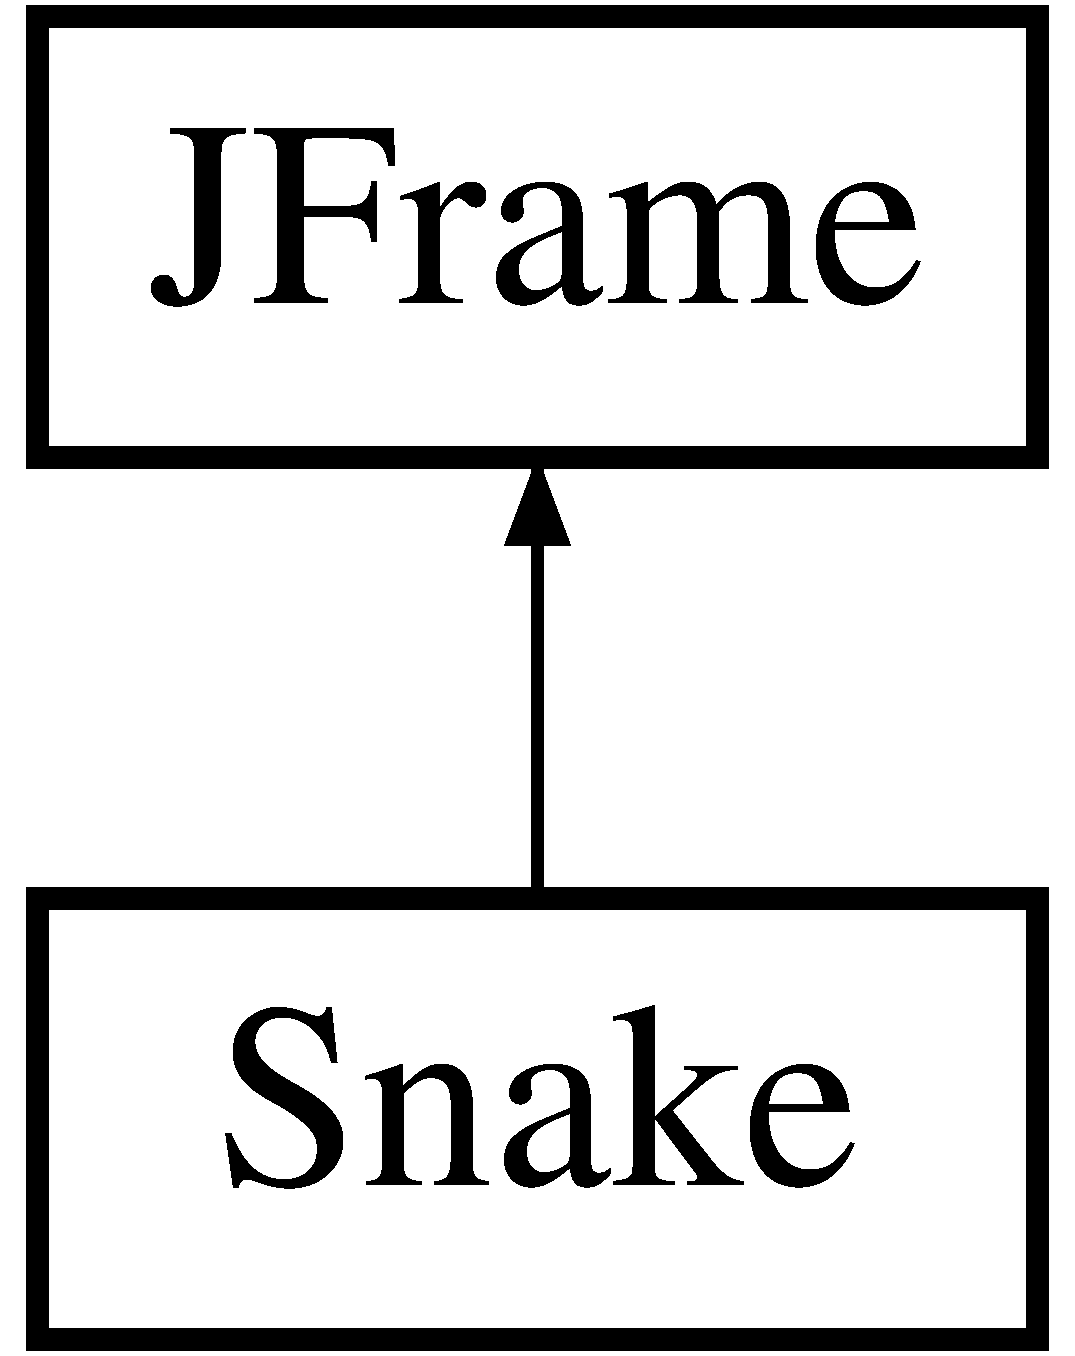
\includegraphics[height=2.000000cm]{class_snake}
\end{center}
\end{figure}
\subsection*{Public Member Functions}
\begin{DoxyCompactItemize}
\item 
\hyperlink{class_snake_a35a64028a338e45a72fadb6ce16ec6bd}{Snake} ()
\end{DoxyCompactItemize}
\subsection*{Static Public Member Functions}
\begin{DoxyCompactItemize}
\item 
static void \hyperlink{class_snake_a44187b37496c7c746cf12abdbf85c8cd}{main} (String\mbox{[}$\,$\mbox{]} args)
\end{DoxyCompactItemize}


\subsection{Constructor \& Destructor Documentation}
\mbox{\Hypertarget{class_snake_a35a64028a338e45a72fadb6ce16ec6bd}\label{class_snake_a35a64028a338e45a72fadb6ce16ec6bd}} 
\index{Snake@{Snake}!Snake@{Snake}}
\index{Snake@{Snake}!Snake@{Snake}}
\subsubsection{\texorpdfstring{Snake()}{Snake()}}
{\footnotesize\ttfamily Snake.\+Snake (\begin{DoxyParamCaption}{ }\end{DoxyParamCaption})}

Constructor for \hyperlink{class_snake}{Snake}. Sets up board, title of window, etc. 

\subsection{Member Function Documentation}
\mbox{\Hypertarget{class_snake_a44187b37496c7c746cf12abdbf85c8cd}\label{class_snake_a44187b37496c7c746cf12abdbf85c8cd}} 
\index{Snake@{Snake}!main@{main}}
\index{main@{main}!Snake@{Snake}}
\subsubsection{\texorpdfstring{main()}{main()}}
{\footnotesize\ttfamily static void Snake.\+main (\begin{DoxyParamCaption}\item[{String \mbox{[}$\,$\mbox{]}}]{args }\end{DoxyParamCaption})\hspace{0.3cm}{\ttfamily [static]}}

Main method to run the game. 
\begin{DoxyParams}{Parameters}
{\em args} & \\
\hline
\end{DoxyParams}


The documentation for this class was generated from the following file\+:\begin{DoxyCompactItemize}
\item 
Snake.\+java\end{DoxyCompactItemize}

%--- End generated contents ---

% Index
\backmatter
\newpage
\phantomsection
\clearemptydoublepage
\addcontentsline{toc}{chapter}{Index}
\printindex

\end{document}
